% Aquí se expondrá todo lo investigado con OpenAI y los modelos de lenguaje.

\chapter{Análisis y evaluación de la práctica con diferentes interfaces en OpenAI}
\label{chap:interfaces_openai}


% \defaultFontEpigraph{Hopfield Network Is All You Need}{\cite{ramsauerHopfieldNetworksAll2021}}
% \defaultFontEpigraph{Hopfield Network Is All You Need}{Ramsauer y cols. (2021)}
\defaultFontEpigraph{Attention Is All You Need}{\cite{vaswaniAttentionAllYou2017}}

La investigación presentada se detalla a continuación, siguiendo la secuencia cronológica del proceso exploratorio realizado con las herramientas proporcionadas por OpenAI. Inicialmente, se examinó ChatGPT, el chatbot desarrollado por OpenAI, para después avanzar hacia el \emph{Playground} y, por último, hacia la \gls{api}. Esta última herramienta ofrece la capacidad de integrar los modelos en entornos de programación personalizados, facilitando la automatización de solicitudes a los modelos y el procesamiento de resultados específicamente en el ámbito de la generación sonora y musical.

A lo largo de las distintas fases de este estudio, se investigó cómo la aplicación de variadas estrategias de \emph{prompting} afecta la precisión y calidad de las respuestas obtenidas de los modelos. Paralelamente, se han evaluado diversas opciones de interfaces de usuario para optimizar la interacción con los modelos, buscando equilibrar usabilidad con eficacia en la generación de resultados.

\section{ChatGPT, como primer banco de pruebas}
La divulgación de las capacidades de los modelos de lenguaje al público general ha sido principalmente a través de chatbots. Aunque actualmente existen numerosos chatbots que incorporan modelos de lenguaje, ChatGPT de OpenAI fue uno de los primeros en ser presentado públicamente. Utilizando actualmente las versiones GPT-3.5 y GPT-4, este chatbot permite entablar conversaciones en lenguaje natural y, aunque hoy en día posee una amplia gama de funciones que lo posicionan como una herramienta útil en diversos sectores para potenciar la productividad, originalmente fue diseñado con el objetivo más simple de facilitar diálogos interactivos.

ChatGPT ha servido en este trabajo como plataforma experimental para investigar el potencial de estos modelos en la esfera de la creación sonora mediante lenguajes de programación, dando una idea clara de cómo avanzar en interfaces más complejas con el uso de la \gls{api}.

\subsection{GPT-4, modelo utilizado en todos los experimentos}

En la sección \ref{sec:llm_asistentes_creacion_codigo_programacion} se ha expuesto el estado del arte de los modelos de lenguaje aplicados a la creación de código, habilidad esta que constituye una de las más notorias. Al mismo tiempo, se señaló que el modelo más avanzado en la actualidad es GPT-4, de OpenAI\index{OpenAI}. No obstante, se realizaron pruebas con otros chatbots, como Bard, de Google, o el mismo GitHub Copilot, cuyos \gls{llm} han recibido un \emph{fine-tuning} específico para la creación de código con todos los repositorios de GitHub. Sin embargo, en GPT-4 se ha encontrado un buen equilibrio entre precisión en respuestas y posibilidades de uso, especialmente gracias a la \gls{api} y su extensa documentación. La Figura \ref{fig:GPT4_correction_comparation} muestra un ejemplo, realizado al azar, que pone de manifiesto la diferencia entre la corrección de código en SuperCollider de GPT-4 y Bard\index{Bard}, en el que se puede apreciar cómo el código generado por este último no se puede ejecutar por sus numerosos errores sintácticos, mientras que el de GPT-4 es correcto. En cuanto al modelo exacto de GPT-4, si bien este ha ido cambiando a lo largo del tiempo en el que se han realizado el trabajo, la versión más utilizada, tanto por coste como por optimización, ha sido \texttt{gpt-4-1106-preview}, más conocida como \emph{GPT-4 turbo}.

A priori se han descartado los modelos open source, ya que demandan, en el momento del trabajo, una gran cantidad de recursos que quedan fuera del alcance de esta investigación. Por otra parte, la aplicación de estos modelos a la generación de código está en pleno desarrollo y, por lo general, aún quedan lejos de las capacidades de GPT-4.

% \footnote{En el momento en el que se está finalizando este trabajo, se ha liberado el modelo open source {Code LLaMa 2}, del que se anuncia un rendimiento superior a GPT-4 \citep{roziereCodeLlamaOpena}.}.


\begin{figure}[h]
    \caption[Respuesta de {Bard} y {ChatGPT} a un mismo prompt]{(\textbf{a}) Respuesta de {Bard} y (\textbf{b}) {ChatGPT} a un mismo prompt: <<Haz un código sencillo en SuperCollider, listo para ejecutarse, que ejemplifique una frecuencia modulada>>. El código de {Bard} cuenta con varios errores graves de sintaxis, mientras el de {ChatGPT} es correcto.}
    \centering
    \begin{subfigure}{.48\textwidth}
    \centering
    \begin{lstlisting}[style=SuperCollider-IDE, basicstyle=\footnotesize\ttfamily, numbers=none]
// Declaramos las variables
float fm = 440;
float fms = 100;
float amp = 0.5; 

// Generamos la señal FM
SinOsc s = SinOsc(fm);
s.freq = 
s.freq * (1 + fms * SinOsc(fms).cos);

// Asignamos la señal a un bus
Out(s);
    \end{lstlisting}
    \caption{Bard (con Palm 2)}
    \end{subfigure}\hfill
    \begin{subfigure}{.48\textwidth}
    \centering
    \begin{lstlisting}[style=SuperCollider-IDE, basicstyle=\footnotesize\ttfamily, numbers=none]
(
SynthDef(\fmSimple, {
    |out = 0, freq = 440, 
    modIndex = 10,
    modFreqRatio = 1|
    var modulator = 
    SinOsc.ar(freq * modFreqRatio) 
    * modIndex;
    var carrier = 
    SinOsc.ar(freq + modulator);
    Out.ar(out, carrier ! 2);
}).add;
)

// Tocar el SynthDef
(
Synth(\fmSimple, [
    \freq, 440,   
    \modIndex, 20, 
    \modFreqRatio, 0.5
]);
)
    \end{lstlisting}
    \caption{ChatGPT (con GPT-4)}
    \end{subfigure}

    \source{\propio}
    \label{fig:GPT4_correction_comparation}
\end{figure}


Un segundo \gls{llm} disponible en ChatGPT, GPT-3.5, si bien es capaz de generar código mejor que el de Bard, no lo hace con la tasa de corrección de GPT-4. En los experimentos realizados esto se pudo comprobar constantemente: una gran parte del código generado en SuperCollider por GPT-3.5 contenía demasiados errores de sintaxis y alucinaciones, lo cual lo convertía en ineficiente para la creación de código musical al lado de GPT-4.


\section{Rendimiento de ChatGPT en tareas de generación de código sonoro}
Por la propia interfaz de chatbot, ChatGPT solo permite una interacción tipo \emph{diálogo}. Esto es, el usuario introduce un texto, y el modelo responde a este texto. Esto determina fuertemente el tipo de tareas que con él podemos realizar a la hora de crear código musical. No resulta práctico para la creación de código musical en tiempo real, ya que es el usuario quien debe cortar y pegar constantemente texto desde el IDE al chat y viceversa, lo cual entorpece el flujo de trabajo. Sin embargo, se ha visto muy útil para las tareas que enumeramos a continuación:

\begin{itemize}
    \item Crear esbozos generales de una obra.
    \item Crear bloques de código sencillos.
    \item Poner a prueba ciertas técnicas de prompting, como \gls{cot}.
\end{itemize}

\subsection{Creación de esbozos generales de una obra}
Una de las tareas más útiles que se ha encontrado para ChatGPT en relación con la composición musical es la de crear esbozos generales de una obra. Esto es, estructuras generales, como la forma temporal, junto con la estructura del código con las clases y funciones que eventualmente se van a usar. Se trata de una planificación previa a la composición de los detalles. En este punto es tentador pensar que ChatGPT podría producir la obra completa, pero esta ilusión cae rápidamente al intentarlo, ya que lo más probable es encontrar multitud de errores en el código generado, los cuales provienen de una mala planificación general y no merece la pena depurar. Sin embargo, si el objetivo de una conversación es simplemente la de crear una estructura general, el resultado puede ser satisfactorio.

Para llevar a cabo una tarea así, se ha encontrado conveniente hacer que nuestro prompt pida al \gls{llm} realizar una planificación previa de la obra de forma razonada, siguiendo técnicas de prompting como \gls{cot} (véase sección \ref{sec:llm_tecnicas_prompting}). En este sentido, se ha visto muy útil que el prompt contenga una serie de indicaciones que guíen al modelo en la creación de la estructura general de la obra. Por otra parte, la mayor parte de las veces que se le ha pedido este tipo de trabajo, lo ha hecho correctamente solo tras iterar ciertas indicaciones en la conversación.  Por ejemplo, en el prompt de la Figura \ref{fig:ChatGPT_esbozo_estructura} se puede ver cómo se le pide al modelo que cree una estructura general de una obra. Su primera respuesta, a pesar de ser correcta desde el punto de vista del lenguaje, no responde en absoluto a la dimensión temporal pedida, que es la esencia de la estructura. Pero simplemente devolviéndole una pista de lo que se busca, su segunda respuesta se adecua perfectamente a lo pedido originalmente. 

Ya desde el inicio de los experimentos se ha visto que el \emph{feedback} del usuario experto en la tarea pedida es fundamental para no frustrar la tarea inmediatamente. Sin embargo, llama la atención que ChatGPT no comprenda la esencia de la petición primera, en el ejemplo dado, la de crear una estructura temporal esquemática, y que baste una pista para que la respuesta sea correcta. Este hecho apunta a que la iteración es la clave para obtener buenos resultados. Los \gls{llm} \emph{razonan} mejor en conversaciones, donde pueden ir recibiendo \emph{feedback} del usuario, que en prompts aislados.


\begin{figure}[H]
    \caption[Conversación con ChatGPT para crear una estructura general de una obra]{Conversación con ChatGPT para crear una estructura general de una obra. El prompt (\textbf{a}) pide al modelo que cree una estructura general de una obra de unos 5 minutos de duración. La respuesta ignora la dimensión temporal pedida, por lo que se le da una pista de lo que se busca. La respuesta al siguiente prompt (\textbf{b}) se adecua perfectamente a lo pedido originalmente.}
    \centering
    \setstretch{1}
    \begin{subfigure}{.48\textwidth}
    \centering
    \begin{lstlisting}[style=SuperCollider-IDE, basicstyle=\footnotesize\ttfamily, numbers=none]
// Definición de SynthDef 
para la introducción
SynthDef(\granularSynth, { 
    |out = 0, freq = 440, dur = 1|
    // Código para síntesis granular
}).add;

// Patrón para la sección de introducción
Pbind(
    \instrument, \granularSynth,
    \dur, Pwhite(0.1, 0.3),
    \freq, Pexprand(400, 500)
).play;
    \end{lstlisting}
    \caption{Respuesta a \emph{Prompt} 1: <<Crea la estructura en SuperCollider de una obra de música electroacústica.  La duración ha de ser de unos 5 minutos. El desarrollo temporal ha de ser la de una modificación constante de la textura sonora. Ayúdate de las técnicas de síntesis sonora que sean necesarias en cada caso. El código ha de ser modular. Los detalles se trabajarán después. Interesa un adecuado uso de las clases y \emph{placeholders} de SuperCollider. Haz primero una planificación razonada.>> Nota: se han eliminado los comentarios previos al código de las respuestas.}
    \end{subfigure}\hfill
    \begin{subfigure}{.48\textwidth}
    \centering
    \begin{lstlisting}[style=SuperCollider-IDE, basicstyle=\footnotesize\ttfamily, numbers=none]
// Definición de secciones como funciones
~introduccion = {
    // Código para la introducción
    "Iniciando introducción".postln;
    // Duración de la introducción
    60.wait;
};

~desarrollo = {
    "Iniciando desarrollo".postln;
    120.wait;
};

~climax = {
    "Iniciando clímax".postln;
    60.wait;
};

~conclusion = {
    "Iniciando conclusión".postln;
    60.wait;
};

// Secuenciador temporal con Routine
Routine({
    ~introduccion.value;
    ~desarrollo.value;
    ~climax.value;
    ~conclusion.value;
}).play;
    \end{lstlisting}
    \caption{Respuesta a \emph{Prompt} 2: <<Utiliza algún tipo de rutina para organizar el aspecto temporal.>>}
    \end{subfigure}
    \source{\propio}
    \label{fig:ChatGPT_esbozo_estructura}
\end{figure}

Una vez que ChatGPT nos ha provisto de un esqueleto para una obra musical, ¿por qué no continuar la conversación hasta tener todas sus partes completas? Los intentos de crear códigos completos desde cero, paso a paso, han sido casi siempre frustrados en algún punto de la conversación. Llegados a una cierta cantidad de peticiones y respuestas, puede resultar desconcertante el olvido del  \gls{llm} de ciertos aspectos importantes del trabajo realizado en la misma conversación hasta el momento y el que queda por completar. 


Esto se debe a varios factores: En primer lugar, la ventana de contexto definitivamente limita la memoria del \gls{llm} (el número de tokens que recibe como input para la siguiente respuesta) de forma que los primeros prompts, precisamente en los que se le daban las directrices generales para una obra, quedan fuera de su alcance. Su comportamiento en ese momento es impredecible, y tiende a enfocarse en las últimas tareas como objetivo principal. Y debido a que el usuario desconoce cuál es el valor de esta ventana de contexto, puede arrastrar el proyecto en la conversación hacia un punto sin salida. En segundo lugar, independientemente de la ventana de contexto, y especialmente en las ventanas grandes, se ha visto que los \gls{llm} no procesan por igual toda la información. Pueden existir lagunas importantes en el centro de la ventana, tal como se vio en la sección \ref{sec:hiperparametros_ventana}, lo cual contribuye a que una conversación lo suficientemente larga pueda derivar a un bloqueo o a un caos, especialmente cuando el usuario, como en el caso de los chatbots, desconoce el tamaño de la ventana en la conversación.

\subsection{Creación de bloques de código sencillos}

Nos referimos con \emph{bloque sencillo} a una pieza de código funcional, pero que no constituye un proyecto completo, como, por ejemplo, una función, un patrón, etc., con unas pocas líneas de código. Al no constituir un código de una obra completa, no se requiere del manejo de una gran información en las respuestas del \gls{llm}, por lo que se puede esperar una mayor precisión en las mismas, al tiempo que se evitan los problemas asociados con la ventana de contexto. Del mismo modo, se ha comprobado que el usuario, a priori, puede controlar mejor así la conversación, iterando de una forma más controlada y cómoda. 

Esta forma de trabajo, sin embargo, requiere de una buena planificación por parte del usuario, en la medida en la que es este quien dará unidad a los diferentes elementos del trabajo sonoro y musical. En este sentido, es difícil pensar en un buen rendimiento de este flujo de trabajo sin conocimientos sólidos de las herramientas de programación utilizadas. Si bien existen técnicas de uso de \gls{llm} que implican la interacción de varios modelos o conversaciones paralelas, al modo de \emph{agentes}, en este trabajo no se ha explorado esta posibilidad debido a su complejidad y a la falta de técnicas y plataformas maduras que permitan su uso\footnote{Con relación a técnicas de agentes aplicadas a la generación de código, véase \cite{huangAgentCoderMultiAgentbasedCode2023}. Un repositorio con extensa y actualizada bibliografía sobre el tema puede encontrarse en \cite{AGIEdgerunnersLLMAgentsPapers2024}.}.

En general, en nuestros experimentos se ha encontrado que GPT-4 se ha desenvuelto con notable corrección en sus respuestas en el sentido sintáctico, mostrando una alta capacidad de autocorrección cuando se le ha devuelto un código de error, requiriendo poca o nula intervención humana en la corrección de errores. No obstante, como ocurría en el caso de la creación de esbozos generales de una obra, se han encontrado casos de bloqueo en la conversación, en los que el \gls{llm} no ha sido capaz de avanzar en la tarea sin la intervención humana. 

El lenguaje utilizado para comunicarse con GPT-4 siempre ha sido, deliberadamente, el lenguaje natural, orientado a la creación sonora y musical, con el fin de encontrar así los límites de esta herramienta. Incluso en el caso de conversaciones en las que se devuelve código correcto y funcional, se han encontrado diversos problemas a nivel artístico, que hay que tener muy en cuenta a la hora de utilizar esta herramienta con fines musicales y que pasamos a detallar.

% \begin{itemize}
%     \item Alucinaciones recurrentes.
%     \item Abuso de valores <<por defecto>>, que restan interés artístico al código.
%     \item Errores indetectables y potencialmente peligrosos.
%     \item Introducción de errores de sintaxis en código previamente correcto.
%     \item Ocasionales errores de sintaxis que escapan a la autocorrección.
%     \item Gran distancia entre el sonido producido y el sonido esperado.
% \end{itemize}

\subsubsection{Alucinaciones recurrentes}
Las {alucinaciones} en los \gls{llm} (véase la sección \ref{sec:alucinaciones}) son una de las características más conocidas de estos modelos, al tiempo que una de las más difíciles de detectar sin una supervisión humana, y, por ende, uno de los mayores handicaps a la hora de delegar tareas de cualquier índole a sistemas de IA. En el mejor de los casos estas alucinaciones se producen en el uso de clases o métodos inexistentes en el lenguaje de programación en uso. Normalmente estos defectos son fáciles de detectar por el compilador o por el intérprete del lenguaje, que suele dar cuenta de dicho problema inmediatamente. Por ejemplo, en el caso de SuperCollider, un código como el de la Figura \ref{fig:alucinacion_chatgpt} es correcto desde el punto de vista sintáctico, pero no lo es desde el punto de vista de la semántica del lenguaje, ya que utiliza la clase \texttt{KarplusStrong}, que no existe en SuperCollider. En este caso, el intérprete de SuperCollider dio buena cuenta de este error. 

\begin{figure}[H]
    \caption[Alucinación de ChatGPT utilizando una clase que no existe]{Alucinación de ChatGPT utilizando una clase que no existe ante el prompt <<Crea una textura sonora en supercollider inspirándote en el modelado físico de sonido.>> ChatGPT utiliza como base el UGen \emph{\texttt{KarplusStrong}}, el cual no existe en SuperCollider.}
    \centering
    \setstretch{1}
    \begin{lstlisting}[style=SuperCollider-IDE, basicstyle=\footnotesize\ttfamily, numbers=none]
// Crear una función para el sonido modelado físicamente
(
SynthDef(\ksTexture, {
    arg freq=440, amp=0.5, gate=1, pan=0;
    var env, sig;
    env = EnvGen.kr(Env.adsr(0.01, 0.1, 0.6, 0.4), gate, doneAction: 2);
    // Crear el sonido utilizando KarplusStrong
    sig = KarplusStrong.ar(freq, 0.5, 0.1, 1, env);
    sig = Pan2.ar(sig * amp, pan);
    Out.ar(0, sig);
}).add;
)
    \end{lstlisting}
    \source{\propio}
    \label{fig:alucinacion_chatgpt}
\end{figure}


Encontramos errores aún más sutiles y difíciles de detectar, ya que requieren de un conocimiento profundo del lenguaje de programación en uso y el intérprete no da cuenta de ellos, pudiendo pasar desapercibidos. Esto puede constituir un problema de seguridad. Un ejemplo claro es cuando la amplitud de la salida de audio satura el sistema. Los lenguajes de programación sonora no cuentan a priori con limitaciones de volumen o frecuencia, por lo que un error de este tipo puede provocar daños en el equipo de sonido o en el oído del usuario (véase Figura \ref{fig:amplitud_saturada_chatgpt}). Similar a este error es, en SuperCollider, la acumulación de instancias de un \texttt{Synth} en el servidor de audio, lo cual puede provocar un bloqueo del sistema. En la Figura \ref{fig:error_dificil_detectar_supercollider} se puede ver un ejemplo de este tipo de error. En este caso, el usuario ha tenido que intervenir para corregir el código generado por el modelo. Junto al fenómeno de la alucinación, este tipo de problemas pueden pasar desapercibidos especialmente si no existe un entendimiento profundo del lenguaje por parte del usuario.

\begin{figure}[H]
    \caption[Código saturado en amplitud, generado por ChatGPT]{Código saturado en amplitud, generado por ChatGPT. El código es correcto desde el punto de vista sintáctico, pero la amplitud de la señal de audio satura el sistema. Este tipo de errores no son detectados hasta que se ejecuta el código, y son potencialmente peligrosos para el equipo de sonido o el oído del usuario.}
    \centering
    \setstretch{1}
    \begin{lstlisting}[style=SuperCollider-IDE, basicstyle=\footnotesize\ttfamily, numbers=none]
(
    {
        var x, y, z, a, b, c, d, e, f, g, h, mix;
        
        x = SinOsc.ar((Decay.ar(Impulse.ar([4,4.005]), 1e3*MouseX.kr(0, 1).abs)*50), MouseY.kr(0, 1)).distort;
        y = BPF.ar(Saw.ar([40,40.001]), LFNoise0.kr(128)+1*4e3+146, LFNoise1.kr(1)+1*5e-2+0.01).tanh;
        z = DelayC.ar(LPF.ar(LFNoise0.ar(8)**2 + x.tanh.round(0.05), 6e3), 1, LFNoise0.ar(8!2).range(1e-4, 0.02));
        a = BHiPass.ar(LFNoise1.ar(8)**3, y.midicps, y/2e3, 67-y);
        b = PitchShift.ar(Saw.ar(Demand.kr(Impulse.kr(4), 0, Drand(([-12, -7, 0, 7, 12]+33).midicps, inf)), Decay.kr(Impulse.kr(4), 3)), 7, 2);
        c = Impulse.ar(8)*LFNoise1.ar(2);
        d = Limiter.ar(GVerb.ar(BPF.ar(c, [400, 800], 1/9, 50).tanh, 100, 10), 0.9);
        mix = Mix.new([x, y, z, a, b, c, d]);
        Out.ar(0, Splay.ar(mix));
    }.play;
)
            
    \end{lstlisting}
    \source{\propio}
    \label{fig:amplitud_saturada_chatgpt}
\end{figure}


\begin{figure}[H]
    \caption[Error difícil de detectar en SuperCollider]{Error difícil de detectar en SuperCollider: El \emph{\texttt{Synth}} \emph{\texttt{\textbackslash dual\_osc}} no cuenta con mecanismo de autoliberación, por lo que se acumulan ilimitadas instancias en el servidor de audio llamadas desde el bucle \emph{\texttt{loop}} hasta saturar el sistema. Este código fue creado por ChatGPT y posteriormente autocorregido tras pasarle la información del error.}
    \centering
    \setstretch{1}
    \begin{lstlisting}[style=SuperCollider-IDE, basicstyle=\footnotesize\ttfamily, numbers=none]
(
    SynthDef(\dual_osc, {
        arg out=0, freq1=440, freq2=660, amp1=0.5, amp2=0.5;
        var sig;
        sig = SinOsc.ar([freq1, freq2], 0, [amp1, amp2]);
        Out.ar(out, sig);
    }).add;
    )
    // --- código intermedio omitido por brevedad ---
    {
        loop {
            var freq1, freq2, amp1, amp2;
            freq1 = freqPattern1.next * 400 + 100;
            freq2 = freqPattern2.next * 400 + 100;
            amp1 = ampPattern1.next;
            amp2 = ampPattern2.next;
            Synth(\dual_osc, [\freq1, freq1, \freq2, freq2, \amp1, amp1, \amp2, amp2]);
            0.1.wait;
        }
    }.fork;
)
    \end{lstlisting}
    \source{\propio}
    \label{fig:error_dificil_detectar_supercollider}
\end{figure}

\subsubsection{Tendencia a valores {por defecto}}
Otro defecto observado con relación a los parámetros de los métodos y clases del código generado es la propensión a utilizar valores por defecto. Esto, aunque no compromete la seguridad, resta interés al código generado desde el punto de vista artístico. Los valores por defecto son aquellos que un elemento del código utiliza cuando el usuario no provee de un valor explícito. Por ejemplo, en el caso de SuperCollider, el método \texttt{SinOsc.ar} cuenta con un parámetro \texttt{mul} que, si no se provee de un valor explícito, toma el valor por defecto de $1$; o \texttt{freq}, con el valor por defecto de \SI{440}{\hertz}. Por ejemplo, en la Figura \ref{fig:ChatGPT_valores_por_defecto} se puede ver cómo el modelo utiliza valores por defecto en el código generado, lo cual no es deseable desde el punto de vista artístico.

\begin{figure}[H]
    \caption[Código generado por ChatGPT con utilización de valor de frecuencia de \SI{440}{\hertz}]{Código generado por ChatGPT con utilización de valor de frecuencia de \SI{440}{\hertz}. Este valor por defecto no es una excepción, sino que sistemáticamente se encuentran en los parámetros de los métodos y clases del código generados por ChatGPT. Esto, sin duda, resta interés al código generado desde el punto de vista artístico.}
    \centering
    \setstretch{1}
    \begin{lstlisting}[style=SuperCollider-IDE, basicstyle=\footnotesize\ttfamily, numbers=none]
(
    SynthDef(\fmSound, {
        arg freq=440, amp=0.5, modIndex=5, attackTime=0.01, releaseTime=1;
        var carrier, modulator, env;
    
        // Envolvente
        env = EnvGen.kr(Env.perc(attackTime, releaseTime), doneAction:2);
    
        // Modulador
        modulator = SinOsc.ar(freq, 0, modIndex);
    
        // Portadora
        carrier = SinOsc.ar(freq + modulator) * amp;
    
        // Salida
        Out.ar(0, carrier * env);
    }).add;
    
    // Toca el sonido
    Synth(\fmSound, [
        \freq, 440, // Frecuencia en Hz
        \amp, 0.5, // Amplitud
        \modIndex, 5, // Índice de modulación
        \attackTime, 0.01, // Tiempo de ataque en segundos
        \releaseTime, 1 // Tiempo de liberación en segundos
    ]);
) 
    \end{lstlisting}
    \source{\propio}
    \label{fig:ChatGPT_valores_por_defecto}
\end{figure}



\subsubsection{Introducción de errores de sintaxis en código previamente correcto}
Aunque infrecuente, no menos desconcertante es la introducción impredecible de errores de cualquier tipo en código previamente correcto. Si los errores son de sintaxis, el compilador o el intérprete del lenguaje darán cuenta de ellos, pero si se trata de errores de semántica, como puede ocurrir en casos de alucinaciones, pueden pasar desapercibidos. La introducción de nuevos errores en código previo es un problema que aparece según la conversación, o el tamaño del código, es comparable al tamaño de la ventana de contexto. De nuevo, el nivel de conocimientos de usuario es fundamental para detectar este tipo de errores.


\subsubsection{Ocasionales errores de sintaxis que escapan a la autocorrección}
Una característica interesante de los \gls{llm} es la de la autocorrección. Esto es, si el usuario le devuelve un el mensaje de error dado por el sistema, el modelo intenta interpretarlo corregir el problema en la siguiente respuesta. Sin embargo, factores como la introducción de alucinaciones, problemas con la ventana de contexto o la simple carencia de información de entrenamiento en el problema actual del código, pueden hacer que el modelo no sea capaz de autocorregirse, pudiendo llevar a un bloqueo en la conversación, especialmente si esta se extiende demasiado con relación a su ventana de contexto, lo cual, como vimos, puede producir lagunas de información.


\subsubsection{Gran distancia entre el sonido producido y el sonido esperado}
El poder de los \gls{llm} es del procesar el lenguaje natural y traducir descripciones en código funcional. Si el código requerido es el de una función, digamos, en {Python}, que ha de <<devolver el sumatorio de las entradas>>, el nivel de comprensión requerido al \gls{llm} en dicha transcripción es trivial, en tanto en cuanto la propia descripción es prácticamente un pseudocódigo de dicha función. El desnivel semántico no es comparable cuando lo que pedimos al \gls{llm} es complejo artísticamente, como, por ejemplo, <<crear un sonido rugoso que evolucione temporalmente de una textura granular a un sonido armónico con leves y agradables fluctuaciones de sus componentes parciales>>. En este caso, el \gls{llm} ha de comprender la descripción, traducirla a código y, además, generar un sonido que se adecue a la descripción.  En este caso, el desnivel semántico es mucho mayor, ya que la descripción responde a criterios estéticos y psicoacústicos, por lo que el resultado puede ser muy distinto al esperado. En la Figura \ref{fig:ChatGPT_desnivel_semantico} se puede ver un ejemplo de este fenómeno. Este problema puede ser mitigado en parte con el uso de técnicas de prompting y una continua iteración en la conversación, pero en muchos casos el resultado final el resultado aceptado por el usuario puede estar lejos el esperado, lo cual constituye un problema del que hay que ser conscientes a la hora de usar esta herramienta para la creación musical.

\begin{figure}[H]
    \caption[Desnivel semántico de ChatGPT entre el prompt y el código generado en SuperCollider]{Desnivel semántico de ChatGPT entre el prompt y el código generado en SuperCollider. El código aparentemente representa un conjunto de sonidos naturales de un bosque, pero el resultado es ruido blanco de alto nivel de amplitud, totalmente alejado del significado semántico de la descripción.}
    \centering
    \setstretch{1}
    \begin{lstlisting}[style=SuperCollider-IDE, basicstyle=\footnotesize\ttfamily, numbers=none]
(
    // Definir los componentes del paisaje sonoro
    var arroyo, pajaros, viento, hojas;
    
    // Arroyo: Ruido blanco filtrado
    arroyo = { BPZ2.ar(WhiteNoise.ar(0.3), 1000) };
    
    // Pájaros: Tonos agudos y aleatorios
    pajaros = { SinOsc.ar([4000, 4500].choose, 0, 0.1) * EnvGen.ar(Env.perc(0.01, 0.1), Impulse.kr([5, 7].choose)) };
    
    // Viento: Ruido rosa
    viento = { PinkNoise.ar(0.2) };
    
    // Hojas y Ramas: Ruido blanco con envolventes
    hojas = { WhiteNoise.ar(0.1) * EnvGen.ar(Env.perc(0.005, 0.1), Impulse.kr(10)) };
    
    // Mezclar y reproducir todos los componentes
    { arroyo!2 + pajaros!2 + viento!2 + hojas!2 }.play;
)
            
    \end{lstlisting}
    \source{\propio}
    \label{fig:ChatGPT_desnivel_semantico}
\end{figure}

% La forma de salvar esta inadecuación entre la descripción sonora y el resultado sonoro pasa por la constante iteración entre el compositor y el \gls{llm} en la creación de bloques sencillos de código sonoro. Así, pueden producirse fragmentos de código eventualmente de interés, en muchos casos como serendipia, si bien, al menos en el momento de la realización de este trabajo, esta valoración artística entra ya en la percepción estética y subjetiva del creador humano.


\subsection{Influjo del uso de técnicas de {prompting} en ChatGPT}

En la sección \ref{sec:llm_tecnicas_prompting} se han descrito algunas de las técnicas más relevantes en cuanto al prompting de un \gls{llm}, especialmente las que han presentado buenos resultados en aritmética y generación de código de programación, como \gls{cot}. De igual modo, en \ref{sec:llm_asistentes_creacion_codigo_programacion} se presentaban técnicas avanzadas como \gls{scot} en la generación de código.

A continuación se analiza, de forma cualitativa y descriptiva, el impacto que han tenido diferentes técnicas de {prompting} en las respuestas obtenidas del modelo.

\subsubsection{\emph{Zero-shot} versus \emph{few-shot}}

Aunque ChatGPT está entrenado para establecer conversaciones tipo chat, es susceptible de recibir contextos junto a la petición del usuario con un conjunto de ejemplos de código, para que el modelo pueda aprender de ellos para elaborar su respuesta (véase sección \ref{sec:few_shot_prompting}). En este sentido, se ha encontrado que la presentación de ejemplos de código al modelo tiene un efecto positivo en cuanto estilo y formato del código, incluso en el uso de elementos de programación similares a dichos ejemplos, haciéndolo menos proclive a errores sintácticos. Sin embargo, no se ha hallado que el uso de ejemplos de código mejore sustancialmente la calidad del código generado en el sentido artístico. 

La Figura \ref{fig:chatgpt_zero_shot_vs_few_shot} muestra el resultado de una misma petición a ChatGPT con \emph{zero-shot} y \emph{one-shot}. El resultado es claramente positivo en el segundo caso. Como veremos, este resultado es clave para el éxito en la utilización de técnicas más avanzadas, como \gls{rag}.



\begin{figure}%[H]
    \caption[Comparación de resultados de ChatGPT con  {zero-shot} y {few-shot}]{Comparación de resultados de ChatGPT con (\textbf{a}) {zero-shot} y (\textbf{b}) {few-shot}.}
    \centering
    \begin{subfigure}{.48\textwidth}
      \centering
      \begin{mdframed}
        \setstretch{1}
        \fontsize{9.5pt}{11pt}\selectfont
        Usuario: Crea una textura sonora de interés artístico usando el UGen \texttt{FMGrain} en SuperCollider.
      \end{mdframed}
      \begin{lstlisting}[style=SuperCollider-IDE, basicstyle=\footnotesize\ttfamily, numbers=none]
{
    var dur, dens, fund, form, indx, pan;
    dur = MouseX.kr(0.01, 0.2, 1, 0.01); 
    dens = MouseY.kr(20, 50, 1, 0.1);
    fund = 200;                     
    form = 800;
    indx = 2;
    pan = LFNoise2.kr(0.5).range(-1, 1); 

    FMGrain.ar(
        numChannels: 2,
        trigger: Impulse.kr(dens),
        dur: dur,
        carfreq: fund,
        modfreq: form,
        index: indx,
        pan: pan
    )
}.play;    
                \end{lstlisting}
                \captionqr{\emph{Zero-shot} en una petición de creación sonora en SuperCollider}{\emph{Zero-shot} en una petición de creación sonora en SuperCollider.}{https://drive.google.com/file/d/13AMMKehJHzlI8CQUqCqoWMHZ9AI2YgcS/view?usp=drive_link}{audio}
    \end{subfigure}\hfill
    \begin{subfigure}{.48\textwidth}
      \centering
      \begin{mdframed}
        \setstretch{1}
        \fontsize{9.5pt}{11pt}\selectfont
        Usuario: Crea una textura sonora de interés artístico usando \texttt{FMGrain} en SuperCollider. Te paso un ejemplo de uso:
        \begin{lstlisting}[style=SuperCollider-IDE, basicstyle=\footnotesize\ttfamily, numbers=none]
SynthDef(\fm_grain_test, {arg gate = 1, amp = 1;
    Out.ar(0,
        FMGrain.ar(Impulse.ar(20), 0.2, 440, 200,
            LFNoise1.kr(1).range(1, 10),
            EnvGen.kr(
                Env([0, 1, 0], [1, 1], \sin, 1),
                gate,
                levelScale: amp,
                doneAction: 2)
        )
    )
}).add;
s.sendMsg(\s_new, \fm_grain_test, a=s.nextNodeID, 0, 1, \amp, 0.1);
        \end{lstlisting}
      \end{mdframed}
    %   \caption{SuperCollider}

        \begin{lstlisting}[style=SuperCollider-IDE, basicstyle=\footnotesize\ttfamily, numbers=none]
SynthDef(\fm_grain_artistic, { arg gate = 1, amp = 1;
    var sound, freq, dur, pan, rate, index;

    // Parámetros modificables para la textura
    freq = LFNoise1.kr(0.5).range(200, 1000);
    dur = LFNoise2.kr(0.1).range(0.1, 0.5); 
    pan = LFNoise2.kr(0.2).range(-1, 1); 
    rate = LFNoise1.kr(0.3).range(5, 50); 
    index = LFNoise1.kr(0.4).range(100, 800); 

    // Creación de la textura sonora
    sound = FMGrain.ar(
        Impulse.ar(rate), dur, freqindex, 5,pan               
    );

    // Aplicación del envolvente y salida
    Out.ar(0,
        Pan2.ar(
            sound * EnvGen.kr(
                Env([0, 1, 0], [0.1, 0.1], \sin, 1),
                gate,
                levelScale: amp,
                doneAction: 2
            ),
            pan
        )
    );
}).add;
s.sendMsg(\s_new, \fm_grain_artistic, a=s.nextNodeID, 0, 1, \amp, 0.1);              
        \end{lstlisting}
        \captionqr{La misma petición con un ejemplo \emph{Few-shot}}{La misma petición con un ejemplo \emph{Few-shot}. El resultado sonoro es más interesante desde el punto de vista artístico.}{https://drive.google.com/file/d/1C7FDkH706e1OMlcOWrG4qsCoC7Au8GaU/view?usp=drive_link}{audio}
    \end{subfigure}

    \source{\propio}
    \label{fig:chatgpt_zero_shot_vs_few_shot}
\end{figure}

\subsubsection{\emph{Chain of Thoughts} (CoT) y \emph{Structured Chain of Thoughts} (SCoT)}

Esta técnica requiere de un nivel mayor de abstracción en el razonamiento del \gls{llm}, al exigirle una planificación previa a la implementación del código. Esto implica la elaboración de la respuesta en dos pasos, una para la planificación y razonamiento, y otra, para la implementación en sí. Dichos pasos pueden ser dados en una sola respuesta o en dos. En el caso de ChatGPT, o el de cualquier chat de \gls{ia}, a cuyos parámetros de respuesta no podemos acceder, conviene hacerlo en dos respuestas consecutivas para asegurarnos de no alcanzar un límite de tokens en la única respuesta. 

A diferencia de \emph{few-shot}, esta técnica no mejora la respuesta del \gls{llm} de forma drástica, pero sí que se aprecian cambios positivos en cuanto a la complejidad de elementos que el código puede llegar a utilizar. Así, una petición compleja del usuario tiene más probabilidades de éxito si el \gls{llm} tiene la posibilidad de \emph{razonar} previamente los pasos a dar que si lo implementa directamente. A cambio, puede introducir más errores en el código, que el usuario ha de corregir por sí mismo o llevar al \gls{llm} en una conversación iterada. Esta técnica es más apropiada que \emph{few-shot} en el caso de buscar un código para una pieza en evolución temporal, donde se implican estructuras tipo rutinas, patrones y cambios de parámetros o sintetizadores a lo largo del tiempo, aunque, será útil en cualquier aplicación en la que se busque complejidad. En los experimentos realizados se han desechado muchas conversaciones completas por llegar a momentos de bloqueo, en los que la complejidad del código era tal que su depuración era más costosa que la elaboración del mismo a partir de partes más pequeñas.

No se ha mostrado como relevante el uso de una técnica tipo \gls{scot}, en la que el primer paso ha de realizarse en pseudocódigo en lugar de en lenguaje natural. La hipótesis que lanzamos para este resultado es que, a diferencia de las tareas de programación a las que esta técnica originalmente se dirige, el diseño de sintetizadores no requiere de tanta complejidad como una función en Python o C++ que se descompone en flujos como bucles y condicionales. En este sentido, el propio script en SuperCollider se representa a sí mismo y no tiene sentido planificar en un pseudocódigo.

\subsubsection{Técnica de \emph{self-debugging}}

Una aproximación para intentar minimizar los errores sintácticos del código generado podría ser el ya expuesto \emph{self-debugging}, en el que el \gls{llm} ha de dar un paso posterior a la implementación en código para revisar los posibles errores del código. En ninguno de los casos que se ha utilizado se han corregido errores algunos. La única forma de que el \gls{llm} corrija sus errores es que el usuario le devuelva el mensaje de error del compilador o del intérprete del lenguaje, en cuyo caso el \gls{llm} comprenderá el problema y tratará de resolverlo en la siguiente respuesta. 

De hecho, este es un flujo habitual en el que se desenvuelve las conversaciones de creación sonora con ChatGPT. La inmensa mayoría de los bloques de código generados con éxito en este trabajo, han sido realizados de forma iterativa, limpiando el código a partir de los mensajes de error devueltos por el intérprete de SuperCollider. En este punto, el papel del usuario compositor y su nivel de conocimientos es fundamental para el éxito de la tarea. La Figura \ref{fig:iteracion_depuracion} muestra este proceso en bucle en el que el usuario devuelve al \gls{llm} los mensajes de error iterativamente.

\begin{figure}[H]
    \caption[Iteración de depuración de código con ChatGPT]{Iteración de depuración de código con ChatGPT. El usuario devuelve al LLM los mensajes de error iterativamente.}
    \centering
    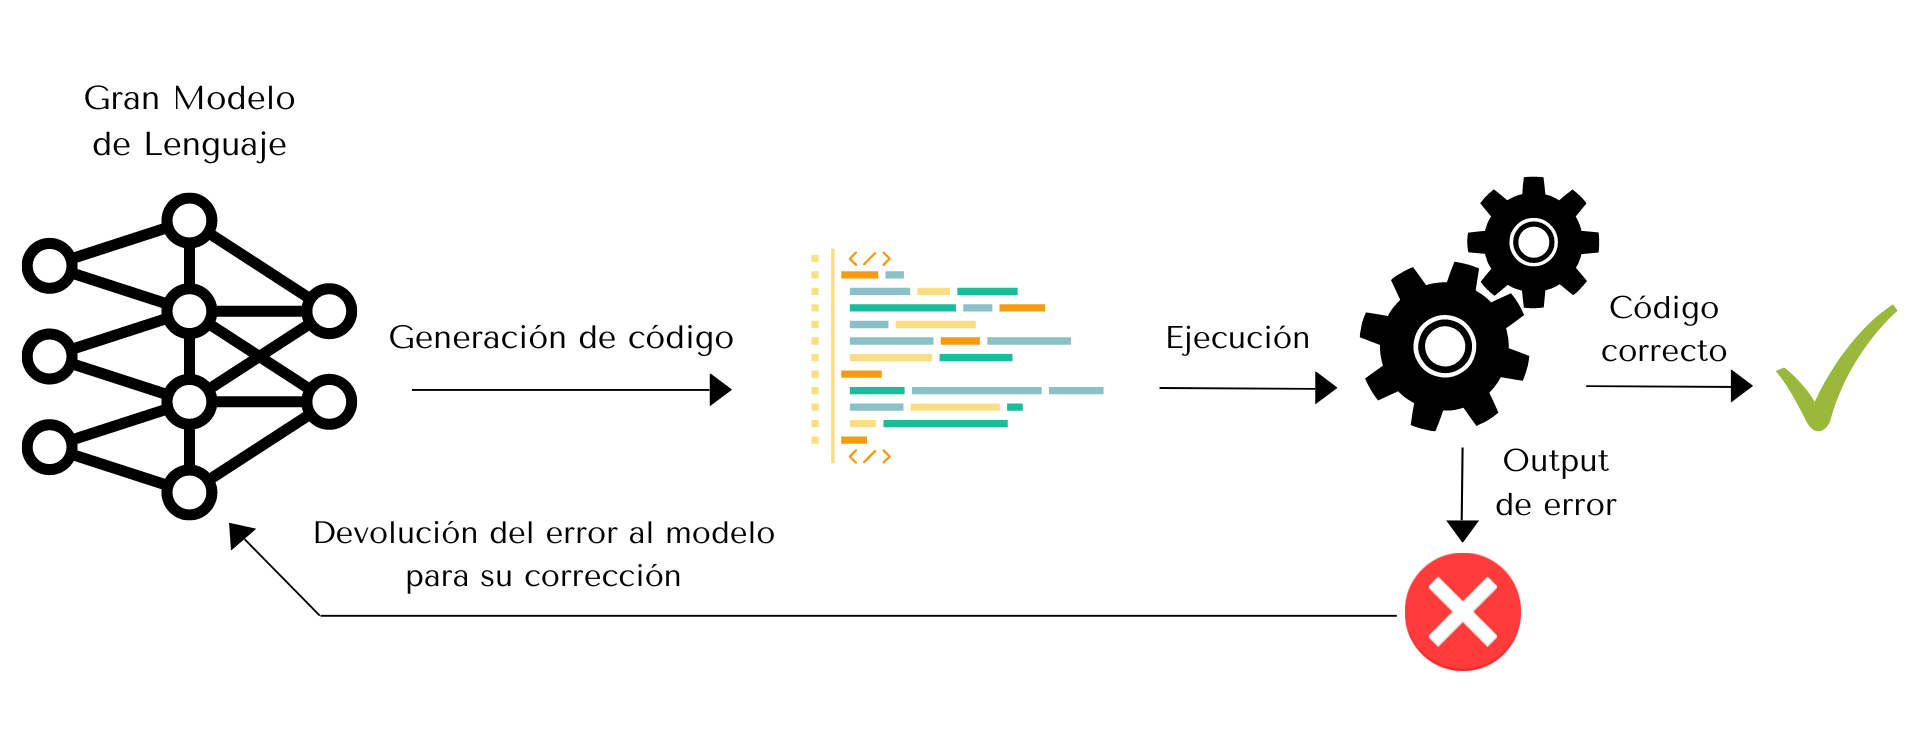
\includegraphics[width=0.9\textwidth]{./figuras/iteracion_depuracion_codigo.png}
    \source{\propio}
    \label{fig:iteracion_depuracion}
\end{figure}

\section{Mayor control de parámetros con el Playground de OpenAI}

El Playground de OpenAI consiste en una interfaz web, similar a ChatGPT, en la cual, entre otras cosas, se pueden controlar importantes parámetros como la temperatura, la longitud de la respuesta, la ventana de contexto, top-\emph{k} y top-\emph{p}. 

En la práctica, se ha visto que no conviene modificar la temperatura más allá de su valor por defecto $1$. Incluso valores ligeramente altos producen efectos negativos en la generación de código, especialmente errores sintácticos y alucinaciones. Valores menores son posibles, aunque estos se tornan demasiado predecibles, y esto puede ser un problema si se busca variedad en las respuestas.

Una ventaja práctica que se ha encontrado en la interfaz de Playground es la posibilidad de escribir un prompt de sistema. Es decir, un prompt general que siempre antecede a los mensajes del usuario. Estos prompts de sistema tienen como finalidad contextualizar la conversación y el papel que el \gls{llm} tendrá dentro de ella. Estos prompts, redactados en lenguaje natural, son una suerte de instrucciones que el usuario puede escribir una sola vez, pero que se espera que el \gls{llm} respete en la conversación. Se ha notado, no obstante, que no siempre son respetadas estas instrucciones, y que prompts de sistema demasiado largos pueden caer en los defectos asociados a la ventana de contexto ya señalados en la sección \ref{sec:hiperparametros_ventana}. La Figura \ref{fig:system_prompt_example} muestra un ejemplo de prompt de sistema utilizado en los experimentos, en el que se le pide GPT-4 que genere código en SuperCollider. Más ejemplos de prompts de sistema utilizados en este trabajo se pueden encontrar en la Figura \ref{fig:system_prompts_aimuse}.

\begin{figure}[H]
    \caption[Ejemplo de prompt de sistema para generar código en SuperCollider]{Ejemplo de prompt de sistema para generar código en SuperCollider. Este prompt ha sido construido iterativamente según las necesidades de la conversación. Muchas instrucciones corresponden a defectos que el LLM ha ido mostrando previamente.}
    \centering
    \begin{mdframed}
        \setstretch{1}
        \fontsize{9.5pt}{11pt}\selectfont
        Eres un experto en SuperCollider. Cada vez que se te pida, debes devolver una sentencia de SuperCollider (SC). Una sentencia puede ser una sola línea o un conjunto de líneas dentro de un bloque. A cada petición, responderás con una única sentencia que continúe el contexto proporcionado por la conversación. Si un usuario reporta un error en tu sentencia, debes corregirla.
        \setlength{\parskip}{6pt}
        Importante: Utiliza Pbindef (no Pbind) como base para la creación musical.
        
        Evita usar el Synth default. En su lugar, crea tus propios SynthDef, asegurándote de:
        1. Evitar valores predeterminados (como "freq=440") y 
        2. Que los SynthDef se autoliberen con "doneAction: 2". 
        Crea patrones, ritmos, texturas, planos sonoros y espacializaciones experimentales. Utiliza siempre la sintaxis correcta de SC y no incluyas texto o comentarios, ya que no serán procesados.
        
        Organiza tus respuestas de la siguiente manera: primero s.boot; luego, define SynthDefs; después, trabaja con Pbinds; y finalmente, termina con s.freeAll y s.quit. Evita bloques de código largos.
    \end{mdframed}
    
    \source{\propio}
    \label{fig:system_prompt_example}
\end{figure}


\section{Ampliando el \emph{Knowledge}: \emph{retrieval-augmented generation}}

OpenAI provee de las herramientas necesarias para implementar sistemas de \gls{rag} (véase sección \ref{sec:rag}), bajo el nombre de \emph{GPTs} y \emph{Assistant}, lo cual fue explorado en el transcurso de la investigación. Básicamente, se ha de proveer al sistema de un prompt de sistema y de un conjunto de archivos sobre los que pueda realizar consultas. 

Para ello, se elaboró una serie de archivos de texto plano a partir de la documentación oficial de las clases de SuperCollider y su guía práctica de uso de \emph{patterns} \citep{SuperCollider12Help}\footnote{Los archivos generados ad hoc para estos sistemas se encuentran en el repositorio del trabajo (véase el anexo \ref{anexo:repositorio})} convertido a formato JSON para facilitar su lectura al sistema. Otro archivo incluido, esta vez en PDF, es el manual \emph{A Gentle Introduction To SuperCollider} de \citeauthor{ruviaroGentleIntroductionSuperCollider2015} (\citeyear{ruviaroGentleIntroductionSuperCollider2015}). Para el caso de los trabajos con el lenguaje de Tidal Cycles, se prepararon en archivos de texto los ejemplos de los cursos disponibles en la web oficial del lenguaje \citep{TidalCycles}.

Por lo general, no se ha encontrado una gran diferencia de calidad en el código generado con \gls{rag}. En los sistemas dirigidos a Tidal Cycles se observó que los códigos generados estaban inspirados en ejemplos reales de código, con las transformaciones pertinentes, aunque probablemente se deba a que los experimentos realizados en Tidal Cycles fueron realizados en el contexto de \emph{live coding}, como se verá, donde el sistema podía tomar al azar códigos para su contexto. Por otra parte, los archivos utilizados para Tidal Cycles contenían básicamente ejemplos de código con un comentario cada uno, mientras que los de SuperCollider contenían más texto, lo cual puede haber influido en el resultado.


\section{Programando con la API de OpenAI}

La comunicación por \gls{api} con los servicios, en este caso, de OpenAI, constituye la forma más dúctil de interactuar con los modelos de \gls{ia}. En este caso, se provee de una amplia y completa documentación y de librerías para su utilización dentro de diversos lenguajes de programación. En nuestro caso, el lenguaje utilizado es Python, por la sencillez de su uso y por ser un lenguaje robusto en el campo de la \gls{ia} y de la investigación. El entorno de programación fue durante toda la investigación Visual Studio Code. Se crearon principalmente dos programas para la interacción con la \gls{api} de OpenAI: uno para la generación automática de código en Tidal Cycles y otro para la generación interactiva de código tanto en Tidal Cycles como en SuperCollider.

\subsection{Generación automática de código en Tidal Cycles}
\label{sec:generacion_automatica_codigo_tidal_cycles}

La \gls{api}, además de interacciones del mismo tipo que ChatGPT o que la Playground, permite la interacción programada de peticiones y la gestión de las respuestas de forma automatizada. Uno de los primeros scripts que se crearon en este trabajo realizaba peticiones cíclicamente a la \gls{api}. El código solicitado era el de un patrón de Tidal Cycles por medio de una petición de prompt de sistema. Una vez obtenido, el patrón es enviado al generador de sonido de Tidal en local y, tras un tiempo determinado, se vuelve a comenzar el ciclo enviando una nueva petición que incluye tanto el prompt de sistema como los patrones que se han generado hasta el momento como contexto.

Una parte de estos patrones generados contienen errores en el código, normalmente por la utilización de objetos o clases inexistentes. En estos casos, como ya se ha mencionado, el error puede pasar desapercibido y sin consecuencias graves en la salida del sonido. Tidal no para la ejecución de los patrones previos aunque el último ejecutado contenga errores. El resultado sonoro del script es el de una evolución temporal de patrones, en forma de deriva, que solo puede ser controlado, en parte, por el usuario desde el prompt de sistema. El resultado es similar al de un intérprete de \emph{live coding} escribiendo código musical en vivo. 

Los resultados obtenidos con esta forma de interacción mostraron una notable diferencia tanto en lo cuantitativo como en lo cualitativo respecto a técnicas previas. Por una parte, el flujo continuo de peticiones a la \gls{api} permite obtener una cantidad de código mayor que con las interfaces tipo chatbot, lo cual se muestra útil a la hora de buscar variedad y cierta serendipia en la búsqueda artística de sonidos y texturas. Por otra parte, la posibilidad de ejecutar directamente el código generado abre la puerta a la experimentación en tiempo real y abre ilimitadas posibilidades en el campo de la música en vivo.

Una decisión que resultó muy productiva es la de utilizar el lenguaje de Tidal en lugar del de SuperCollider. Además de la fácil y silenciosa gestión de errores de Tidal, por tratarse de un lenguaje expresamente diseñado para la creación musical en tiempo real, su código resulta potencialmente menos peligroso que el de SuperCollider, como también se señaló más arriba. 

Las limitaciones de esta forma de interacción se encuentran en la forma de implementación de la interacción con el usuario, que, en este caso, se ha visto reducido absolutamente al prompt inicial. Esto provoca que no exista dominio temporal del flujo. Esta situación se puede solucionar, en parte, programando diversos prompts de sistema para ser lanzados en momentos determinados de la ejecución, aunque esto no fue explorado lo suficiente.

Precisamente, para posibilitar un control mayor por parte del usuario, se creó un segundo programa que permitiera una interacción mucho más directa y abierta, en términos de posibilidades, con la \gls{api}. Debido a la importancia de este programa y su complejidad, se le dedicará un apartado propio (véase capítulo \ref{chap:ai_muse}).
